\chapter{Simulation eines einzelnen Teilchens im harmonischen Potenzial}

Um sich mit dem Simulationsframework vertraut zu machen, wird zuerst ein einzelnes Teilchen im harmonischen Potential simuliert. Die Simulation erfolgt dabei nur in einer Dimension auf der x-Achse. Das verwendete Potential hat die Form
\begin{equation}
V(x) = \frac{1}{2}\epsilon x^2
\end{equation}
Die daraus resultierende Kraft auf ein Teilchen an der Position $x$ l�sst sich wie folgt beschreiben:
\begin{equation}
F(x) = -\frac{\partial}{\partial x} V(x) = -\epsilon x
\end{equation}

\section{Analytische L�sung}
F�r den Fall, dass keine weiteren Kr�fte auftreten, l�sst sich folgende Bewegungsgleichung formulieren:
\begin{equation}
\ddot{x} + \omega^2x = 0
\end{equation}
In dieser Gleichung wurde $\omega = \sqrt{\frac{\epsilon}{m}}$ eingef�hrt. Unter Verwendung der Startbedingungen $x_0=A$ und $v_0=0$ ergibt sich die bekannte L�sung des harmonischen Oszillators, wobei $x_0$ die Startposition und $v_0$ die Startgeschwindigkeit beschreiben:
\begin{equation}
x(t) = A\cos(\omega t)
\end{equation}
Eine detaillierte Herleitung ist zum Beispiel bei \cite[Kap. 11.1]{demtroeder2008} zu finden.
F�hrt man zus�tzlich noch eine Reibungskraft der Form $F_R = -R\dot{x}$ ein, ergibt sich folgende Differenzialgleichung:
\begin{equation}
\ddot{x} + \gamma \dot{x} + \omega^2x = 0
\end{equation}
Dabei wurde $\gamma=\frac{R}{2m}$ gesetzt. Bei der L�sung dieser Differenzialgleichung gilt es drei F�lle zu unterscheiden.
\begin{align}
&\gamma<\omega, \textbf{schwache D�mpfung} && x(t) = A e^{-\gamma t}\cos(\omega t) \\
&\gamma=\omega, \textbf{aperiodischer Grenzfall} && x(t) = A(1+\gamma t) e^{-\gamma t} \\
&\gamma>\omega, \textbf{starke D�mpfung} && x(t) = \frac{A}{\alpha} e^{-\gamma t} \left[ \alpha\cosh(\alpha t) + \gamma\sinh(\alpha t) \right]
\end{align}
mit $\alpha = \sqrt{\gamma^2 - \omega^2}$. Die L�sungen entstehen durch Annahme der gleichen Anfangsbedingungen wie weiter oben beschrieben. Eine ausf�hrliche Herleitung kann bei \cite[Kap. 11.3]{demtroeder2008} nachvollzogen werden.

\section{Numerische L�sung}
\label{chap:HarmOsziNumLsg}
Die eben hergeleiteten analytischen L�sungen sollen nun in der Simulation nachvollzogen werden. Dazu werden folgende Parameter gew�hlt:
\begin{compactitem}
	\item $\epsilon = 1$
	\item $m = 1$
	\item $A = 5.61231$
\end{compactitem}
Die Bewegungsgleichung wird mit Hilfe des Eulerverfahrens
\begin{align}
x_{t+\Delta t} &= x_t + \dot{x}_t \Delta t \\
\dot{x}_{t+\Delta t} &= \dot{x}_t + \ddot{x}_t \Delta t 
\end{align}
diskret in $\Delta t$ Schritten integriert. Zuerst werden die Auswirkungen unterschiedlicher $\Delta t$ auf die Trajektorie untersucht.
\begin{figure}[h!]
	\centering
		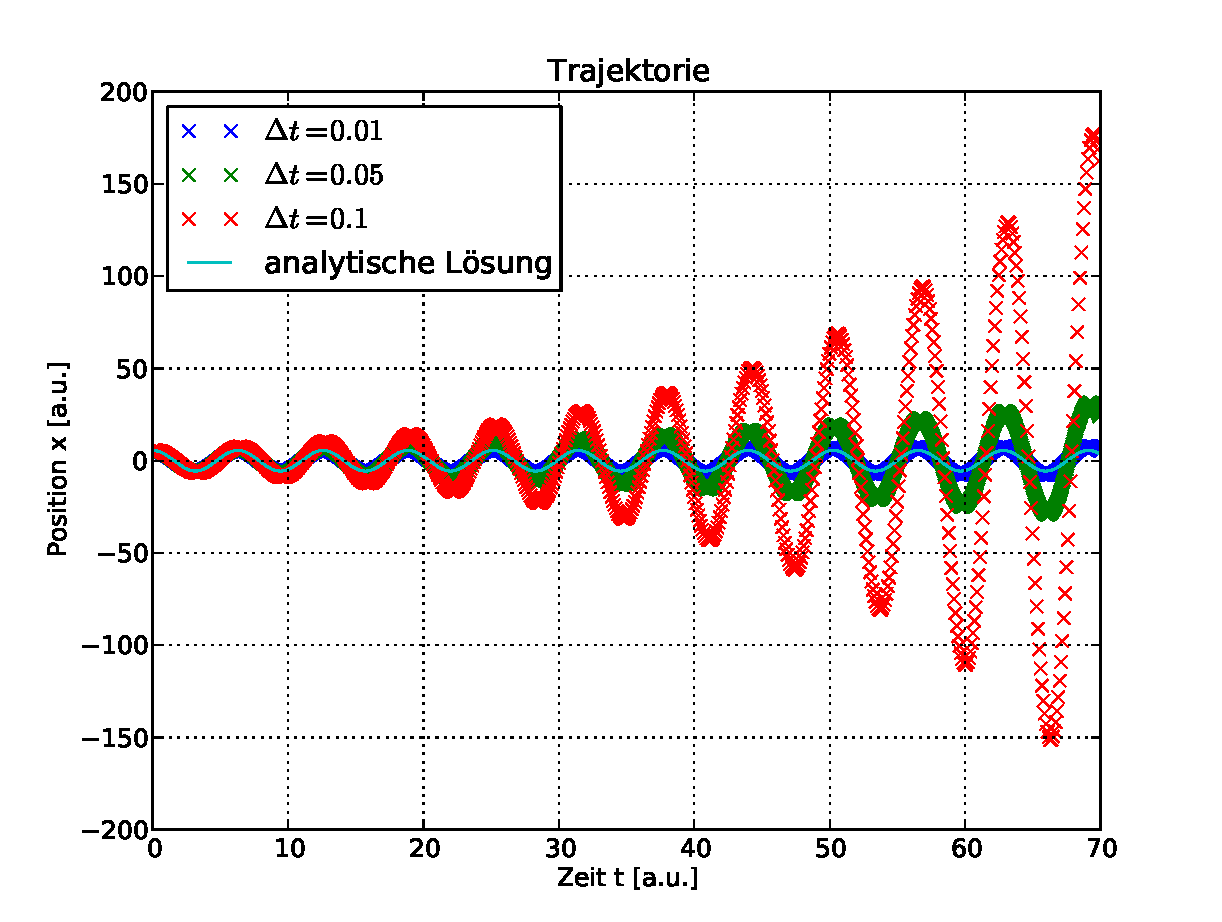
\includegraphics[width=0.70\textwidth]{img/HarmOsziX.pdf}
	\caption{Aufgetragen ist die Position des Teilchens gegen die Zeit. Es zeigt sich, dass das gew�hlte $\Delta t$ signifikanten Einfluss auf die Trajektorie hat. Eine feiner zeitliche Diskretisierung f�hrt zu einem Ergebnis, das n�her an der analytischen L�sung liegt.}
	\label{fig:HarmOsziX}
\end{figure}
F�r unterschiedliche $\Delta t$ lassen sich in \fref{fig:HarmOsziX} deutliche Unterschiede in der Trajektorie feststellen. F�r kleinere $\Delta t$ stimmt der Verlauf besser mit dem theoretisch vorausgesagten �berein. Dies ist nicht verwunderlich, da eine feinere zeitliche Diskretisierung zu kleineren numerischen Fehlern f�hrt. Um die Energieerhaltung des Eulerverfahrens zu �berpr�fen, wird die Energie ebenfalls aufgezeichnet.
\begin{figure}[h!]
	\centering
		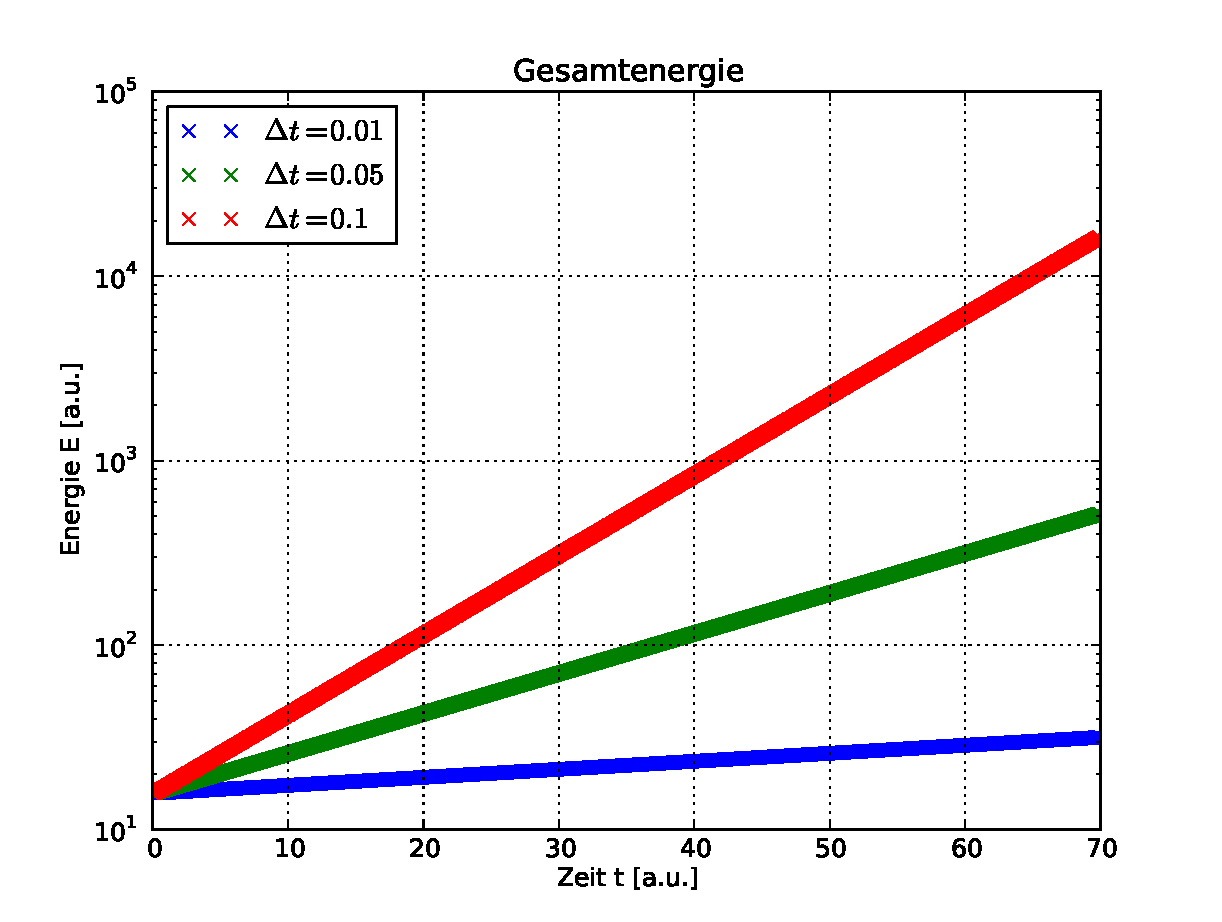
\includegraphics[width=0.70\textwidth]{img/HarmOsziE.pdf}
	\caption{Aufgetragen ist die gesamte Energie des Teilchens gegen die Zeit. F�r die Energieachse wurde eine logarithmische Auftragung gew�hlt, um den exponentiellen Verlauf zu verdeutlichen. Es zeigt sich, dass die Energieerhaltung des Eulerverfahrens sehr schlecht ist.}
	\label{fig:HarmOsziE}
\end{figure}
Die Energieerhaltung ist beim Eulerverfahren nur schlecht gegeben, was man am Divergieren der Energie in \fref{fig:HarmOsziE} erkennen kann. Die St�rke der Divergenz wurde mit Hilfe von Fits ermittelt. Der sich daraus ergebende Zusammenhang ist in \fref{tab:HarmOsziEDivergenz}.
\begin{table}[h!]
	\centering
		\begin{tabular}{c|ccc}
			\toprule
			zeitliche Diskretisierung ($\Delta t$) & 0.1 & 0.5 & 0.01\\
			\midrule
			Proportionalit�t der Energie $\propto\exp (\cdot t)$ & 0.1 & 0.5 & 0.01\\
			\bottomrule
		\end{tabular}
	\caption{Bestimmung der Divergenz der Energie}
	\label{tab:HarmOsziEDivergenz}
\end{table}
Die Werte legen die Vermutung nahe, dass sich die Energie $\propto\exp ((\Delta t) t)$ verh�lt.
Das Eulerverfahren eignet sich also nur bedingt zur Integration von Bewegungsgleichungen, da die Energieerhaltung in der Physik ein fundamentales Prinzip darstellt. Die Fehler k�nnen durch eine feinere zeitliche Diskretisierung verbessert, aber nicht verhindert werden. F�r die F�lle mit D�mpfung zeigt sich ein besseres Bild, da die D�mpfung auch numerische Divergenz der Energie bremst. Da die D�mpfung proportional zur Energie ist, wird in allen F�llen auf 0 ged�mpft. Die Ergebnisse stimmen sehr gut mit den theoretischen Kurven �berein.
\begin{figure}[h!]
	\centering
		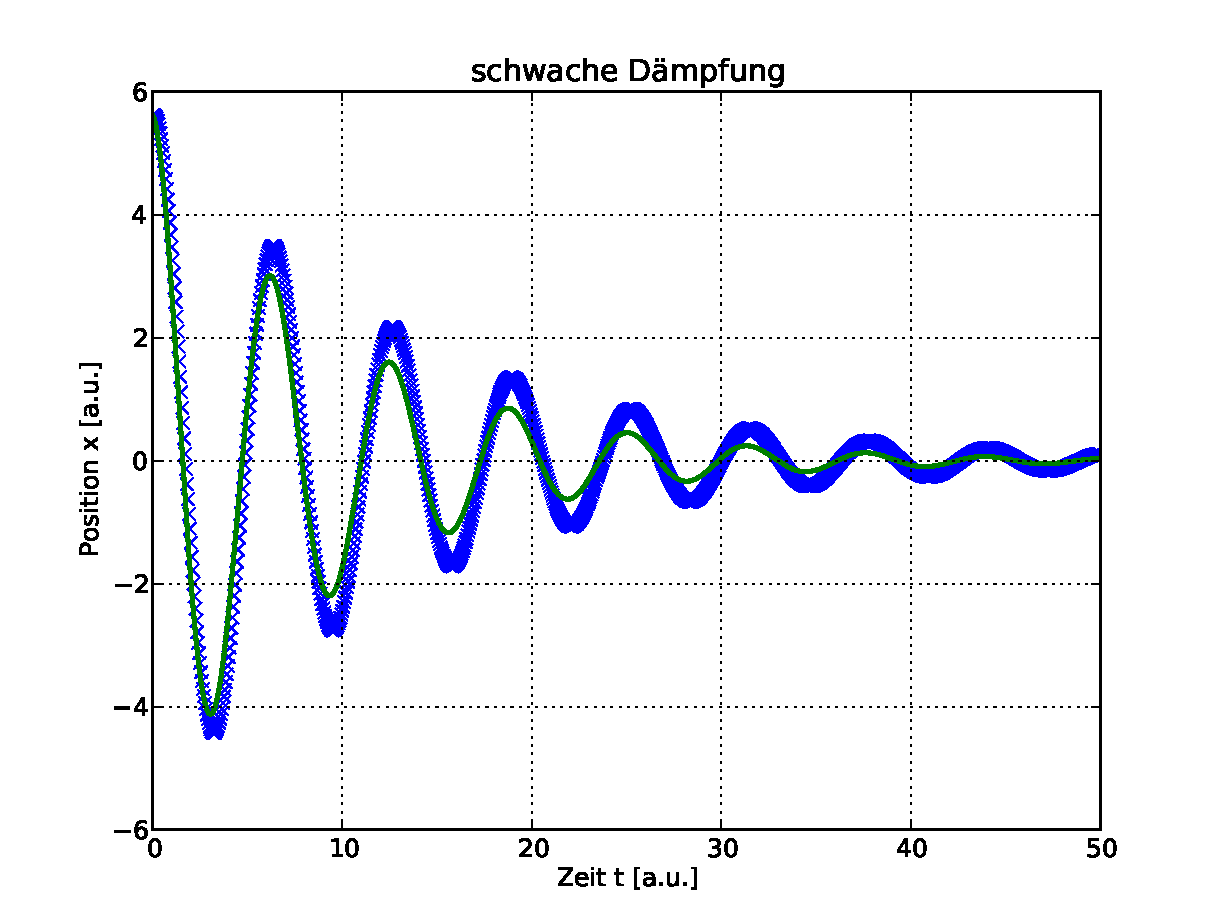
\includegraphics[width=0.70\textwidth]{img/HarmOsziSch.pdf}
	\caption{Harmonischer Oszillator mit schwacher D�mpfung. $\gamma=0.1\omega$. Die simulierte Trajektorie (blau) weicht leicht von der theoretischen Erwartung (gr�n) ab.}
	\label{fig:HarmOsziSch}
\end{figure}
\begin{figure}[h!]
	\centering
		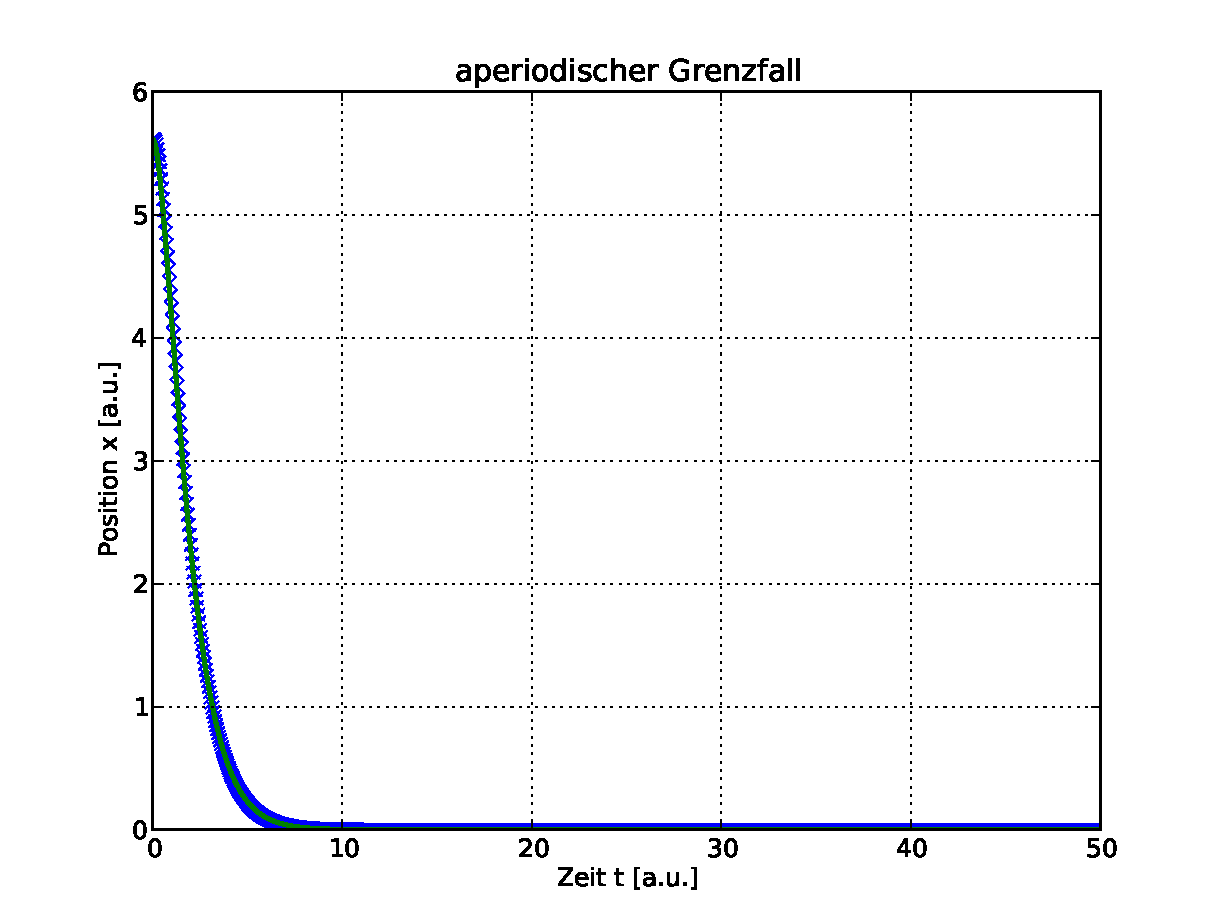
\includegraphics[width=0.70\textwidth]{img/HarmOsziA.pdf}
	\caption{Harmonischer Oszillator im aperiodischen Grenzfall. $\gamma=\omega$.}
	\label{fig:HarmOsziA}
\end{figure}
\begin{figure}[h!]
	\centering
		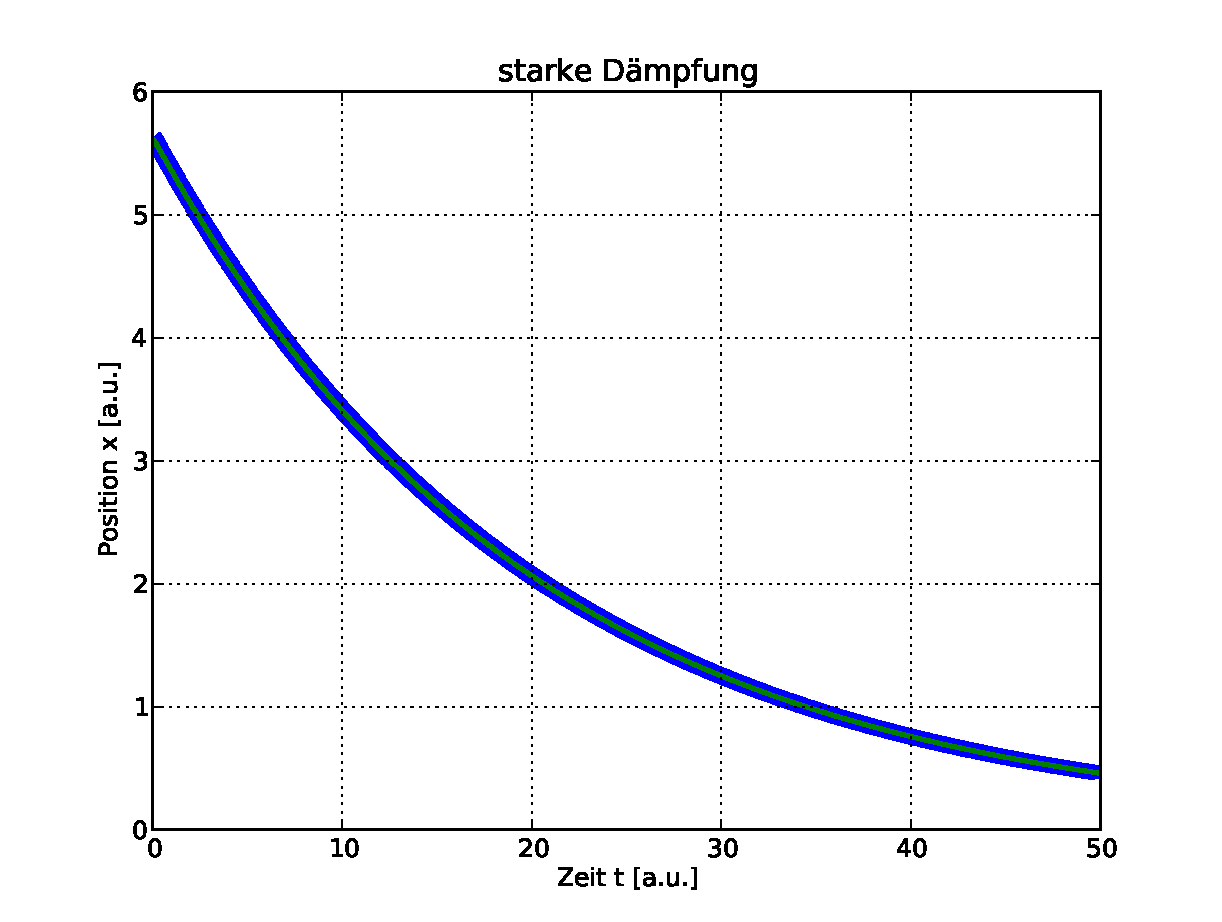
\includegraphics[width=0.70\textwidth]{img/HarmOsziSt.pdf}
	\caption{Harmonischer Oszillator mit starker D�mpfung. $\gamma=10\omega$.}
	\label{fig:HarmOsziSt}
\end{figure}
